\cleardoublepage
\newpage
\ThisULCornerWallPaper{1.0}{chapterimage.eps}
\chapter*{Introdução} % 

%% Usei a mesma estrutura do inicio do quijote
No meu querido povo de Occo, lá na época da minha primeira década, eu vivia dividindo meu tempo entre o trabalho da chacra, meus jogos e os passeios nos serrados.
Os trabalhos no campo, mesmo que pesados para mim, eram possíveis de levar, pois, estes eram feitos com meus pais e irmãos.

Os dias na serra não transcorriam limpos de surpresas, pois de quando em quando, acontecia que algum de nossos animais se perdia; nesses casos, saíamos pelas ladeiras dos montes, gritando os nomes deles, até que escutávamos uma resposta, geralmente em forma de um lamento cheio de saudade.
Esta tática era especialmente eficaz com meu burrinho, pois, ele conseguia escutar meu chamado desde outras montanhas; assim, quando eu gritava seu nome, ele voltava a mim, gritando e chorando, escolhendo seu caminho em função da direção da minha voz.
Em outras ocasiões, percebíamos que desapareciam animais pequenos como frangos ou porquinhos das índias; porém, apos ver as evidências e fazer um trabalho detetivesco, descobríamos que sua ausência era devido à visita de algum falcão, zorro, ou gato de monte.
Nesses casos, só podíamos chorar por eles; mas,  eram poucas as vesses que perdíamos animais dessa forma, pois além das pessoas da casa, tínhamos animais como cachorros e gatos, que aumentavam nosso poder de vigilância.

Minha família não era rica, e talvez esse conceito fugisse do meu entendimento naquela época, mas, nada do que realmente me importava me faltava.
Eu lembro que minha casa era uma cabana de um andar, com teto de palha; minha mãe cozinhava sobre uma fogueira pequena, e meus irmãos e eu, certamente, usávamos com muita frequência roupa que, a simples vista, qualquer pessoa consideraria que eram várias medidas menores das que precisávamos.
Porém, para mim, a minha casa era um castelo amplo e fresco donde ia a descansar após voltar da escola ou de trabalhar na chacra. 
A cozinha da minha mãe era a melhor, cheia de sabores obtidos dos mesmos produtos que cultivávamos ou cuidávamos; em dias especiais meu pai ia ao rio e comíamos peixe, outras vesses na época da seca comíamos carne de sol, e mais comumente alguma mistura de ovos de pato, ou galinha, dependendo da generosidade delas.
Nas nossas refeições não podiam faltar o queijo e a leite, que tanto podiam ser de cabra ou de vaca, pois mesmo tendo só um de cada, conseguiam abastecer á família.
\begin{wrapfigure}{r}{0.35\textwidth}
  \vspace{-10pt}
  \begin{center}
    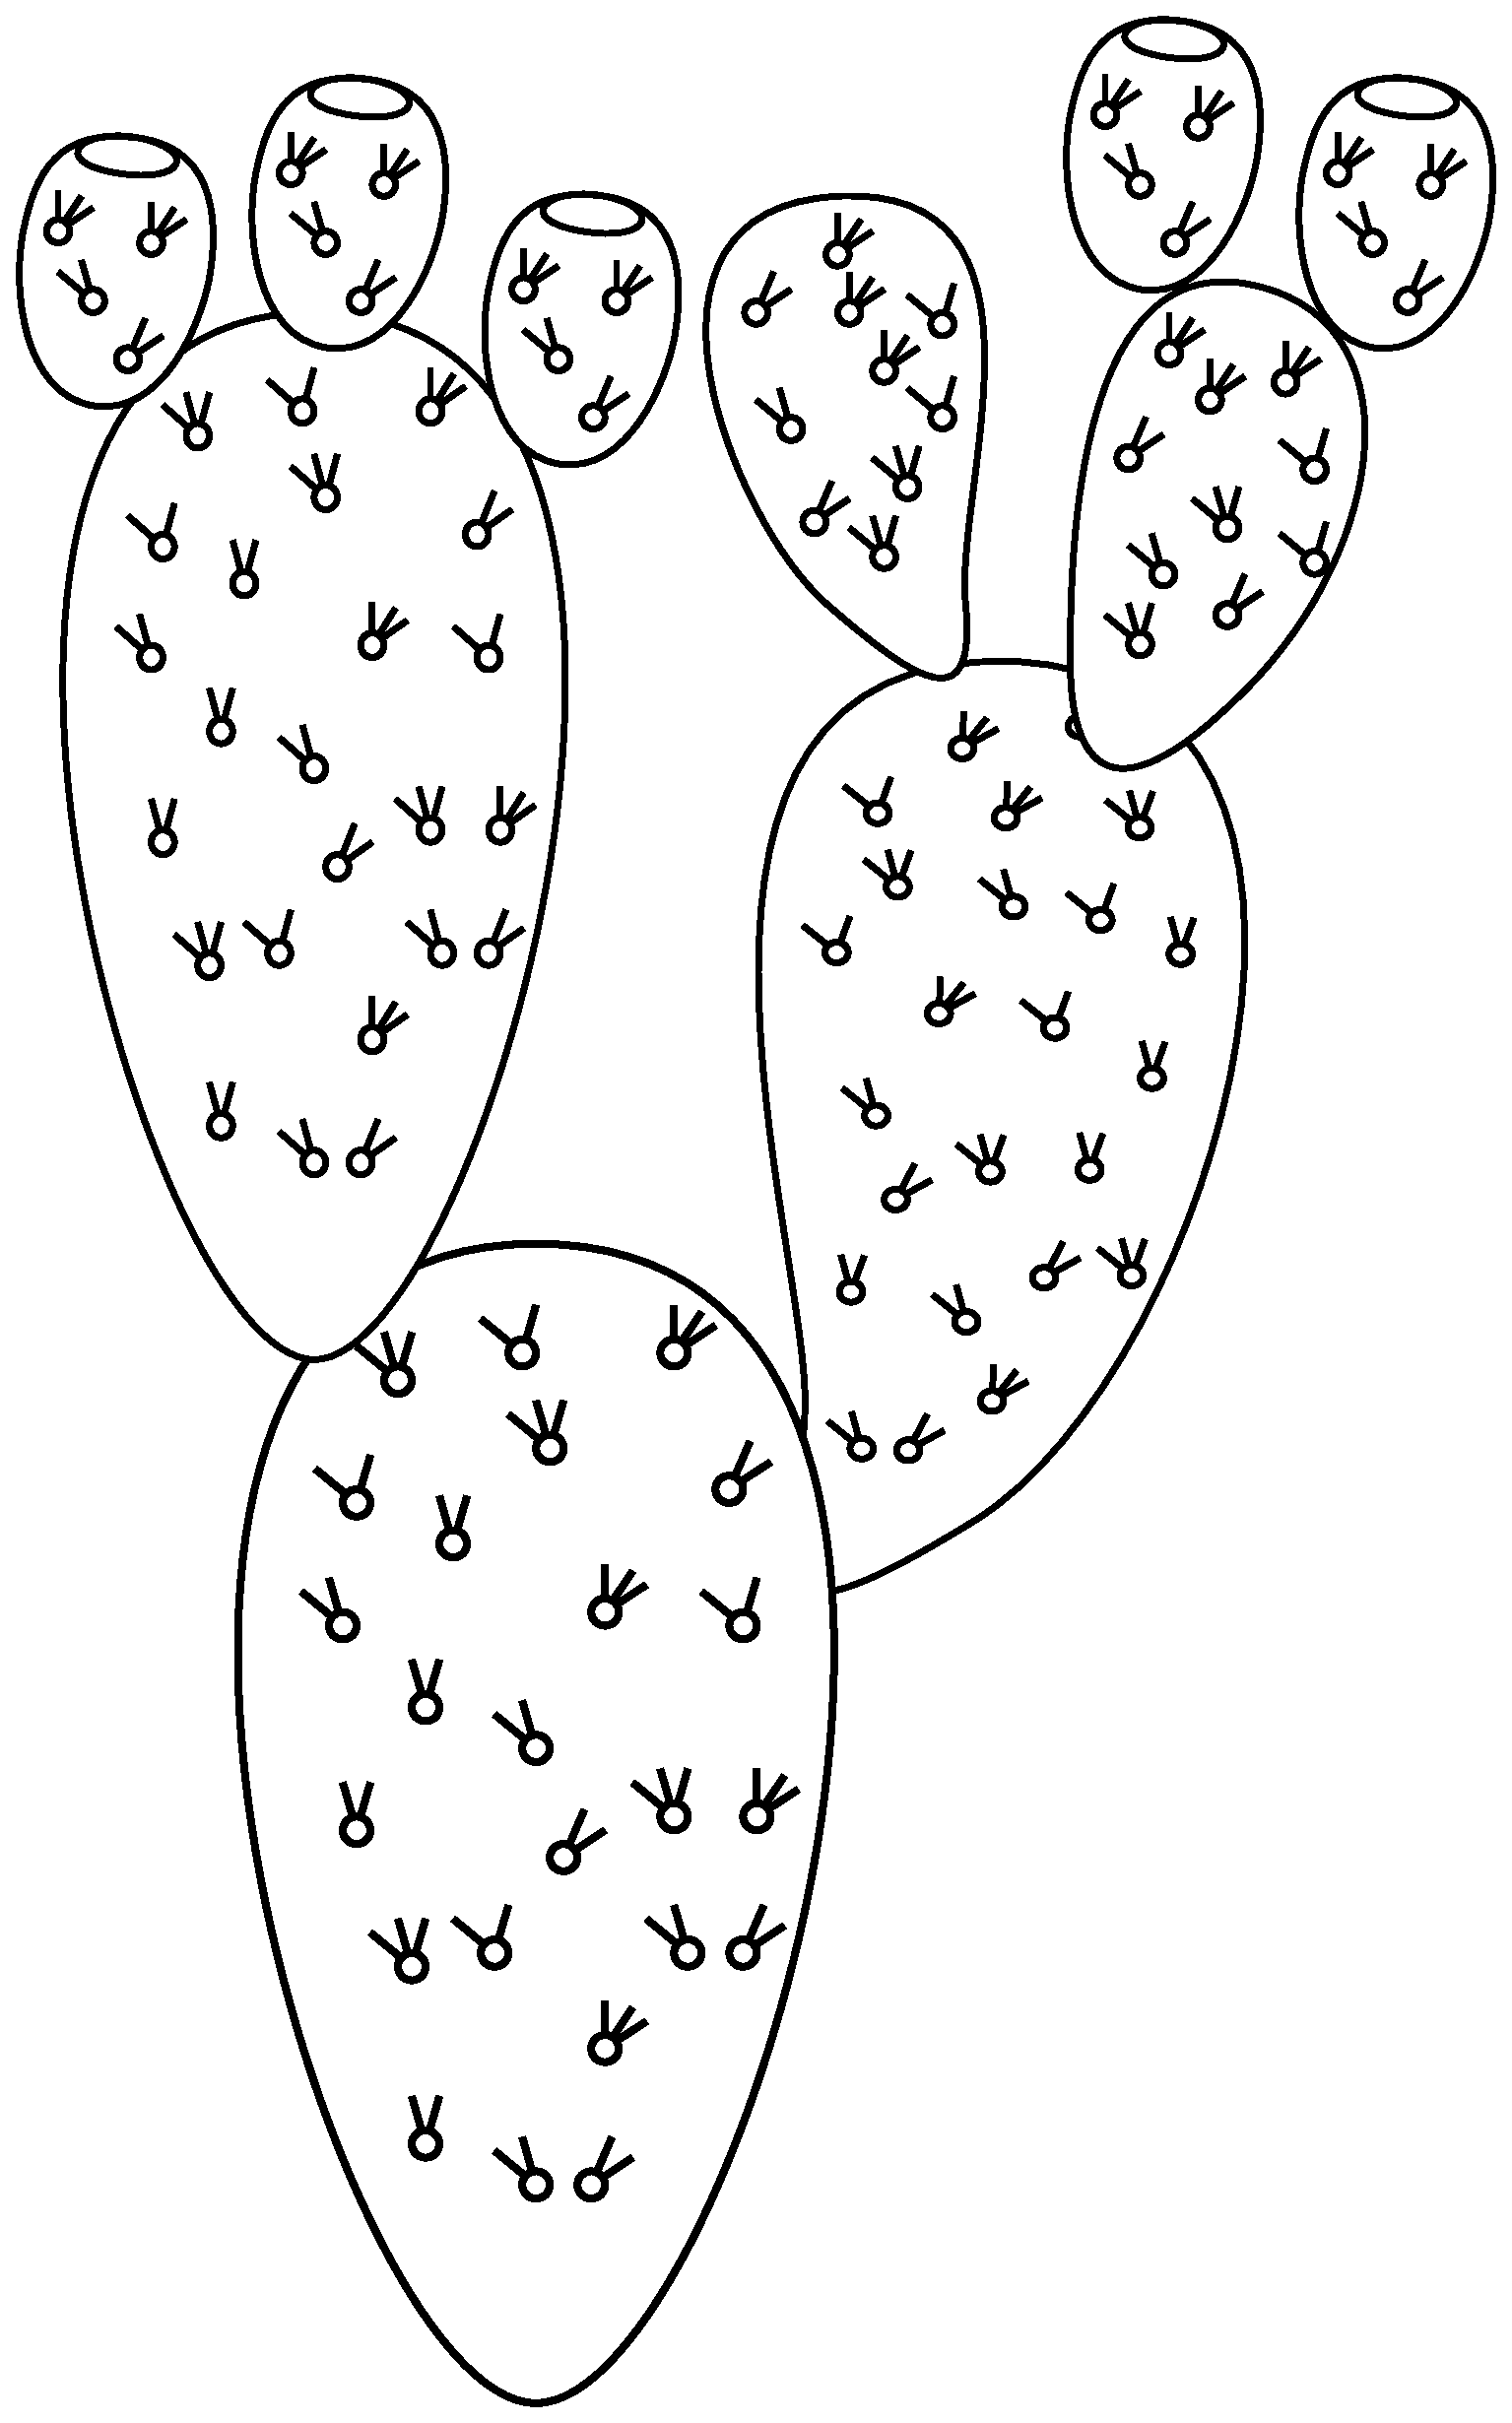
\includegraphics[width=0.30\textwidth]{opuntia.eps}
    \caption{Figo das índias.}
  \end{center}
  \vspace{-30pt}
\end{wrapfigure}
As sobremesas dependiam da estação do ano, pois as frutas como figos das índias, pêssego, figo, melão-andino, sanky, etc. Tinham sua temporada. Também tinham épocas para sobremesas elaboradas com milho fresco, e outras com chila-caiota; com este último minha mãe fazia meu mingau favorito; era inacreditável para mim como com só farinha, açúcar, canela, cravo e chila-caiota, podia ser construído um creme de semelhante majestade.

Meus irmãos e eu gostávamos de brincar juntos, sair a passear procurando obter frutas ou ver animais silvestres; e, em geral, não tínhamos discussões importantes. Meu irmão mais velho tinha um ótimo senso de humor, e costumava me perdoar, mesmo que eu tivesse feito alguma travessura; em verdade, a maioria das vezes, meus problemas eram com minhas irmãs mais novas, pois devo reconhecer que eu costumava fazer alguma maldade.
Nesses casos, elas abriam uma reclamação com as máximas autoridades da casa, com os senhores que governavam e decidiam sobre o bem e o mal, é dizer, meus pais. Lembro que ao princípio meu pai me falava com frases como --- Aurelio, você não deve esconder a boneca da sua irmã --- se a coisa era mais grave ele me falava --- Aule! Porque você colocou o grilo na cabeça da sua irmã? --- e se minha insistência na procura de problemas chegava a níveis perigosos para minha existência, meu pai falava --- \Aulicha! Porque você colocou pimenta na balinha da sua irmã? ---
Assim, quando eu escutava a meu pai me chamar de \Aulicha, eu já sabia que minha sorte já tinha sido decidida e que uma chicotada estava próxima; a ideia de fugir sempre passava por minha cabeça, mas minhas experiências anteriores me indicavam que isso só ia me prejudicar mais, e ia resignado diante do meu pai; inclusive, em várias ocasiões, ele me pedia ir levando esse chicote de três pontas, pequeno e veloz, que era ao mesmo tempo, um velho conhecido e meu principal antagonista.

A minha vida no campo sempre estava cheia de contrapontos, tantos eram os momentos tristes quanto os alegres, e algumas vezes, mas das que me permitiriam pensar que era só uma casualidade, os momentos tristes preparavam um caminho inevitável e irreversível as épocas alegres, e vice-versa; como um ciclo que se retroalimenta para se manter perpetuo. 
Assim, uma das minhas maiores alegrias era quando meu pai retornava de viagem, geralmente da costa do Peru; não só devido à saudade pela partida dele e a alegria pelo seu retorno, mas também porque ele voltava cheio de presentes; trazia doces, bolachas, brinquedos ou roupa; as quais nós na serra não tínhamos acesso comumente.
Por outro lado, entre meus momentos mais tristes, estava a perda de algum ser querido, e minha impotência para evitar sua partida. 
Não entanto, tudo isso é parte da vida, e gostaria compartir com vocês alguns desses momentos.



%Ayacucho é uma cidade do distrito de Ayacucho, na província de Huamanga, no departamento de Ayacucho, no Peru
